\documentclass[a4paper, 12pt, french]{article}

\usepackage{geometry}
\newgeometry{lmargin=3cm}
\newgeometry{rmargin=3cm}

\usepackage[french]{babel}
\usepackage[utf8x]{inputenc}
\usepackage{amsmath}
\usepackage{graphicx}
\usepackage[colorinlistoftodos]{todonotes}
\usepackage{natbib}
\usepackage{titlesec}
\usepackage{multirow}
\usepackage{array}
\usepackage{colortbl}

\usepackage{url}
\usepackage{caption} 
\usepackage{multirow}
\usepackage{adjustbox}
\usepackage{float}
\usepackage{epsf}
\usepackage{longtable}
\usepackage{lscape}
\usepackage[T1]{fontenc}
\title{Rapport de Stage}

\author{Simon Belot}

\date{\today}

\begin{document}

\begin{titlepage}

\newcommand{\HRule}{\rule{\linewidth}{0.5mm}} 

\center 
 
\textsc{\LARGE Stage}\\[0.5cm] 
\textsc{\LARGE (EINGM231)} \\[0.3cm] 
\textsc{\Large Université de Namur }\\[0.3cm]

\HRule \\[0.4cm]
{ \huge \bfseries Rapport de Stage}\\[0.03cm] 
\HRule \\[1.5cm]

\begin{minipage}{0.4\textwidth}
\begin{flushleft} \large
\emph{Réalisé par:}\\BELOT Simon
\end{flushleft}
\end{minipage}
~
\begin{minipage}{0.4\textwidth}
\begin{flushright} \large
\emph{Soumis à:}\\ Prof. John CULTIAUX
\end{flushright}
\end{minipage}\\[1cm]

{\large Mai 2017}\\


\includegraphics[width=10cm, height=10cm]{logounamur.png}\\ 

\vfill

\end{titlepage}

\tableofcontents
\newpage

\section{Situation}

J’effectue mon stage au sein de la société AKABI \footnote{http://www.akabi.eu}. Cette entreprise de consultante a vu le jour au Grand-Duché de Luxembourg en 2011 et a, dès 2012, décidé d’ouvrir une filiale en Belgique. \\

AKABI propose différent services de consultance, de gestion de projets et de formation dans les domaines touchant à l’informatique décisionnelle \footnote{Business Intelligence (BI) en anglais}. En généralisant, on peut dire que l’informatique décisionnelle est un processus de traitement, de stockage et de modélisation de données provenant de différentes sources. L’objectif étant de parvenir à une représentation simple et cohérente de la situation d’une entreprise afin de soutenir la prise de décision. \\

C’est un marché en pleine expansion qui a atteint en 2016 un volume de 16,9 milliards de dollars. Cela représente une augmentation de 5,2\% par rapport à 2015. \citep{ZDNet2016Marche2016}  \\ 

La société AKABI est consciente de cette opportunité et à établi un stratégie claire afin de continuer son expansion :

\vspace{0.25cm}
\begin{itemize}
\item[$\bullet$] Devenir une entreprise de référence en matière de BI sur le marché.
\item[$\bullet$] Assurer une croissance saine (pas de dettes, pas de turnover \footnote{La rotation de l'emploi ou « renouvellement du personnel » est un indicateur décrivant le rythme de renouvellement des effectifs dans une organisation. \citep{WikipediaTurnover}}).
\item[$\bullet$] Se concentrer sur la qualité au lieu de la quantité.
\item[$\bullet$] Assurer le développement personnel et professionnel de chacun.
\end{itemize}
\vspace{0.5cm}

Aujourd’hui, grâce à cette stratégie, l’entreprise emploie une cinquantaine de consultants qui pour la plupart ont des responsabilités au sein de la structure d’AKABI (processus de recrutement, infrastructure, marketing, ...). 

On peut définir un consultant comme un spécialiste extérieur à une organisation à qui l’on fait appel afin d’obtenir un avis au sujet d’une question ou de l’aide pour résoudre un problème précis \citep{GDTConsultant}. Il existe deux raisons principales pour lesquelles des organisations font appel à des consultants. Premièrement lorsqu'un client a besoin d’une personne experte dans un type de travail, dans une phase de développement ou dans une technologie particulière. Dans ce cas la, il fait appel à une société de consultance possédant cette ressource. Deuxièmement, lorsqu'un client a besoin d’une aide temporaire sur un projet qui doit être clôturé dans un certain laps de temps. Dès lors, le client fait donc appel à une société de consultance pour disposer de cette ressource supplémentaire temporairement. \\

Le concept d’informatique décisionnelle peut appliquant à beaucoup de domaines d’activités, c’est la raison pour laquelle AKABI possède un portefeuille de client variée \footnote{http://www.akabi.eu/references/}. 

Pour ma part, j’ai été envoyé en mission au sein du siège de la banque ING Luxembourg. ING (Internationale Nederlanden Groep) est une institution financière internationale d'origine néerlandaise qui offre des services bancaires par le biais de sa société opérationnelle ING Bank et qui détient une part importante dans les compagnies d'assurance NN Group NV et Voya Financial, Inc. B. La branche luxembourgeoise du groupe emploie un effectif de 800 personnes et se classe 11ème employeur du secteur financier du Grand-Duché. Au Luxembourg, ING dispose de 16 agences et de 2 sièges administratifs regroupant les activités de gestion financière, commerciale et administrative de la banque. \\

ING Luxembourg poursuit le développement de ses activités en l’axant sur 3 piliers majeurs : 
\vspace{0.25cm}
\begin{itemize}
\item[$\bullet$] Le réseau local ou « retail banking » (ING occupe une position de challenger au Grand-Duché).
\item[$\bullet$] La banque privée ou « private banking ».
\item[$\bullet$] La banque de l’entreprise ou « corporate banking ».
\end{itemize}
\vspace{0.5cm}

Afin de soutenir son projet de développement, le groupe ING à depuis peu décidé de mettre en place un programme intitulé «Global Data Management» (GDM). Ce programme doit placer les données au centre des préoccupations et créer une source unique et fiable d'information pour toute l’organisation. Cette stratégie devrait permettre d’aider l'ensemble des filiales d'ING à assurer que les données qu'elles fournissent sont exactes, cohérentes et pertinente. 

L'idée de base derrière le programme GDM est de centraliser toutes les soumissions de données dans un seul répertoire et d'établir une définition commune des données au sein d’ING. Cette source unique de données rendra plus efficace la recherche d'information et la génération de rapports, que ce soit en externe auprès du régulateur et de la communauté des investisseurs, ou en interne pour les décisions de gestion, de renseignement client et d'analyse avancée. En plus de cela, le GDM réduira les demandes manuelles, éliminera les interfaces inutiles et améliorera la vitesse et la précision du système pour permettre aux employés de consacrer moins de temps à l'approvisionnement de données et plus de temps à les utiliser. Pour résumer, le GDM vise à construire une base solide pour la nouvelle génération de banques numériques. \\

La stratégie GDM est partagée par toutes les entités du groupe et se base sur 6 éléments concrets:
\vspace{0.25cm}
\begin{itemize}
\item[$\bullet$] Mettre en place une gouvernance de données \footnote{La gouvernance de données associe un ensemble de personnes, de processus et de technologies pour garantir la qualité et la valeur des informations d'une entreprise. \citep{TalendLaDonnees}}.
\item[$\bullet$] Communiquer sur l'importance des données.
\item[$\bullet$] Harmoniser la définition des données.
\item[$\bullet$] Standardiser les architectures techniques
\item[$\bullet$] Améliorer la qualité des données
\item[$\bullet$] Suivre des Data Policies and Privacy
\end{itemize}
\vspace{0.5cm}

Pendant la période de mon stage j’ai principalement travaillé sur le pilier consacré à la qualité de données au sein de l’entreprise. Ce dernier m’a permis d’aborder plusieurs étapes du processus d’informatique décisionnel (recueil des exigences, reporting, communication).

\section{Description de la problématique}

A travers son programme de «Global Data Management», ING veut parvenir à fournir des informations opportunes et précises à ses clients. L’un des plus grands défis pour atteindre cet objectif est, dès lors, la qualité des données générées au sein du groupe. En effet, des données précises permettent la création de rapports de qualité pouvant soutenir la prise de décision. Bien qu’essentiel, mesurer la qualité des données reste un concept vague. C'est la raison pour laquelle il existe plusieurs techniques. La plus couramment utilisée, est celle de "fitness for use", c'est-à-dire une évaluation de la mesure avec laquelle certaines données servent les objectifs de l’utilisateur. \\

Garantir des données précises à chaque étape de l'entreprise est quelque chose de difficile. En effet, de petites erreurs dans la source de données d'origine sont rapidement aggravées lorsqu'elles traversent les différents systèmes et processus d’une organisation. \\ 

ING Luxembourg comme beaucoup d’entreprise à l’heure actuelle, fait face à des problèmes lié à la qualité de ses données. En effet, vu le nombre important de sources d’informations disponibles au sein de l'organisation, un manque de qualité de données est inévitable. 

Le dernier exemple marquant auquel l'entreprise a été confronté est celui concernant les données de nationalité du client. Le département IT, dans lequel j’effectue mon stage, à en effet remarqué il y peu de temps qu’il y avait un nombre anormalement important de client de la banque d’origine népalaise au Luxembourg. Malgré la présence de plusieurs restaurants népalais sur le territoire, il existait une incohérence dans les chiffres. En se penchant sur le problème, les équipes de data management on alors découvert qu’il s’agissait d’un problème d’encodage de données lors de l’enregistrement du client au sein de la banque. \\

Ce manque de précision peut avoir des conséquence importante au niveau du management. En effet, toute incohérence au sein des données engendre inévitablement un manque de précision au moment du reporting et donc se répercute sur la prise de décision (ex: campagne marketing). De plus, étant donné que les entreprises à l'heure actuelle utilise des sources d'information de plus en plus vastes et de plus en plus complexes, ce risque de mauvaise qualité des données ne cesses d'augmenter. \\

\section{Impacts de la problématique}

Un manque de qualité de données au sein d'une entreprise peut entraîner plusieurs types coûts [La mauvaise qualité des données est un problème coûteux : 3 conseils pour progresser]. En effet, des données de mauvaise qualité qui ne sont pas identifiées et corrigées peuvent avoir des répercussions économiques et sociales significative pour une organisation. Cela peut ce traduire par une diminution de la satisfaction client, des coûts de fonctionnement accrus, des processus décisionnels inefficaces et une réduction de la satisfaction professionnelle des employés. De plus, la mauvaise qualité des données augmente les coûts opérationnels car la détection et la correction d'erreurs requièrent des ressources importantes (temps, connaissance, ...). On voit donc bien que les dommages engendré par les données de basse qualité sont vastes et dépendent, entre autre, de la nature et de l'utilisation faite de ces dernières. \\

Bien que les données de mauvaise qualité peuvent impliquer une multitude de conséquences négatives dans une entreprise, on peut regrouper ces coûts en 2 types : 

\vspace{0.25cm}
\begin{itemize}
\item[$\bullet$] Les coûts lié au nettoyage et au maintient de la qualité des données.
\item[$\bullet$] Les coûts engendré par les mauvaises décisions sur base des données de mauvaise qualité. 
\end{itemize}
\vspace{0.5cm}

ING ne déroge pas à la règle et subit inévitablement ces coûts commun à toutes les industries. Néanmoins dans le domaine bancaire, suite à la crise financière de 2007 différentes exigences réglementaires sont apparue afin de renforcer les capacités des banques à faire face au stress et aux situations de crise. La mise en œuvre du principe BCBS (Comité de Bâle sur le contrôle bancaire) n°239 exige par exemple une agrégation efficace des données de risque et un reporting précis des risques. La plupart de ces nouvelles réglementations sont appliquées par les institutions internationales d'importance systémique depuis janvier 2016. Comme la qualité des données a un impact majeur sur les résultats des rapports exigés par les régulateurs, un coût supplémentaire important pourrait concerner les institutions financières en présence de données de basse qualité. \\

Bien que ces coûts sont inévitables, l'estimation exacte de l'ampleur de ces dommage reste difficile. 

\section{Définition de la question}

\begin{center}
\textit{\textbf{"Pourquoi existe-il des données de base qualité dans une institution financière telle que ING Luxembourg?"}}
\end{center}

\section{Convictions}

Cinq grandes pistes de réflexion ont été identifiées. Ces convictions découle d’un travail d’analyse et d’observation réalisé pendant la période de mon stage.

\subsection{Manque d'homogénéité entre les systèmes d’information du groupe ING}

En travaillant au sein de l'entreprise, j'ai pu m'apercevoir qu'il n'existait pas de normes sur les échanges de données entre les différentes entités du groupe ING. Cela entraîne un manque de cohérence au sein de l’organisation entière et par conséquent des problèmes de données de mauvaise qualité. En effet, dans certains cas, des information portant sur le même sujet (ex: TVA) ne sont pas traité de la même manière d'un pays à l'autre (ex: TVA annuelle vs TVA mensuel). Dès lors, l'utilisation de ces données peut engendrer de la confusion lorsque ces dernières sont analysées. \\

Conscient de cette lacune et suite au renforcement des réglementations concernant les données bancaires, le groupe ING à décidé de lancer un programme intitulé «Global Data Management» (GDM) \footnote{http://www.dama-belux.org/wp-content/uploads/2015/03/INGBvdHaarDAMAconference24March-2015.pdf}. L'idée derrière le GDM est de centraliser, au sein de chaque entité, les données dans un répertoire unique et d'établir une définition commune des données à travers l’ensemble de groupe ING. L’objectif de ce dictionnaire de données interne est de s’assurer que tout le monde parle bien de la même chose lors d’un échange d’information au sein de l'organisation. De plus, la source unique de données devrait rendre la recherche d'information et la génération de rapports plus efficaces pour chaque siège d'ING. Il semble en effet indispensable au sein d'une organisation internationale de mettre en place des règles permettant d'avoir une homogénéité au sein des données. \\

L'absence de norme est une source évidente de mauvaise qualité de données. Bien que ce programme n'en soit encore qu'au stade de projet, ce problème devrait être résolus dans les mois à venir et devrait permettre d'améliorer l'échanger et la qualité des données au sein du groupe.

\subsection{La gestion de la qualité des données n'est pas une priorité}

Malgré les initiatives développées par le groupe ING afin de normaliser les échanges de données au sein de l'organisation. La gestion de la qualité des données, bien que évoqué dans le programme GDM, ne semble pas être une priorité actuellement. \\

En effet, même si la majorité du département IT est consciente de l'importance de cette tâche, la direction quant à elle ne semble pas mesurer les conséquences potentiels lié au manque de qualité de données. C’est d’ailleurs la raison pour laquelle, le projet "data quality" a été suspendu pendant un an. En effet, après interview avec plusieurs employés, il ressort que d'autres projets doivent être traité en priorité car ils sont imposés par le groupe. C’est le cas de la mise en place du répertoire unique d’information au sein de l’entreprise, qui devra néanmoins fonctionner avec des données de bonne qualité afin d’être efficace. De plus, il apparaît que les budgets consacré à la réalisation de projet IT soient limités. Raison de plus pour focaliser son attention sur les projets considérés comme cruciaux. \\

Néanmoins, il est possible d’espérer que l’organisation consacre plus d’importance à la qualité des données dans les mois à venir suite à la mise en place de son programme GDM. 

\subsection{Manque de communication interne sur l'importance de la qualité des données}

Un autre point venant appuyer le fait que la qualité des données au sein de l’entreprise n’est actuellement pas une priorité est le fait qu’il existe un manque de communication interne sur le sujet. En effet, une partie de ma mission fût justement d’écrire des «news» \footnote{La communication concernant le programme de gestion de la qualité des données est disponible en annexes.} sur le sujet destinées aux employés d’ING Luxembourg. Ces textes court seront disponibles sur le réseaux interne de la compagnie et devraient permettre d’informer les gens sur l’importance de la qualité des données au sein de l'entreprise. Grâce à cela, le nombre de problèmes liés à un manque de qualité de l’information devrait, au moins au sein de la société, diminuer.

\subsection{Manque de responsabilités concernant la qualité des données}

ING possède également un manque de responsabilité concernant la mauvaise qualité de ses données. En effet, il existe actuellement une lacune dans la gouvernance des données de l'entreprise et plus particulièrement au niveau de la responsabilisation de certaines personnes en temps que ‘’propriétaire’’ \footnote{Le Data Owner ou le propriétaire de la donnée est celui qui détient l’expertise métier pour définir la donnée, sa qualité, ainsi que les moyens pour l’obtenir et la contrôler. \citep{LeJournaldesRHLeCoulisses}} de données. Assigner des responsabilités à certaines personnes devrait permettre de renforcer l'attention portée à la qualité des données. En effet, en cas de problème important avec une de ses données, un "propriétaire de données" devra rendre des comptes et le cas échéant en assumer les conséquences. \\ 

La désignation de data owners fait également partie du programme GDM d'ING. Cela prouve qu'il existe une prise de conscience sur le manque de responsabilités actuelle au sein de l'entreprise. 

\subsection{Le niveau de sécurité informatique complique la résolution de problèmes liés à la qualité des données}

Comme toute institution financières, ING Luxembourg respecte un nombre important de règles et procédure de sécurité qui, suite à la crise financière de 2007 ce sont renforcées. Particulièrement concernant les données manipuler au sein des banques. Bien que maintenir un niveau de sécurité important semble inévitable à l’heure actuelle, ce dernier peu néanmoins compliquer l’identification et la résolution de problèmes liés à la qualité des données. \\

Au sein d'ING les normes de sécurité rendent l’obtention d’accès aux logiciels de gestion de données difficile. J’ai personnellement été confronté à ce problème durant les premières semaines de mon apprentissage. En effet, aucun employés ne semblait savoir qui avait le pouvoir de me fournir les accès aux programmes. Néanmoins ces logiciels de visualisation des données de l’organisation étaient indispensable dans la mission qui m’était attribuée. Sans ces accès, impossible d’identifier et de corriger les problèmes de qualité de données. \\

Le deuxième point important lié à la sécurité et compromettant la gestion de la qualité de données, est le fait que certaines données dites sensibles restent invisibles pour l’équipe data management d’ING. En effet, pour des raisons de confidentialité, certaines information sur les clients de la banque (nom, balance de compte, …) sont cachées dans les différents logiciels et rapports de l’entreprise. Bien que cela soit nécessaire de garantir l'anonymat des clients, ces normes de sécurité engendre des soucis évident d'identification d'erreurs dans les données. En effet, il se pourrait qu’il existe des données de mauvaise qualité mais que ces dernières soient non-identifiables par les équipes IT. \\

Dans les années à venir, le niveau de sécurité exigé au sein des institutions financières ne devrait pas diminuer, bien au contraire. En effet, un nombre toujours plus important de régulations sont mise en place \footnote{Liste non-exhaustive des régulations concernant les données dans le secteur financier disponible en annexes} afin, entre autres, de renforcer l'agrégation des données de risque et les pratiques de déclaration des risques.

\section{Conclusion}

L’analyse de la situation permet clairement de conclure que gestion de la qualité des données n’est actuellement pas assuré de manière optimale au sein d’ING Luxembourg. En effet, il existe plusieurs explications à la présence de données de base qualité au sein d'une institution financière telle que ING Luxembourg. Néanmoins, cette observation à pu identifier plusieurs propositions proposées par l’entreprise afin de tenter de répondre au problème de qualité de données. \\

\vspace{0.25cm}
\begin{itemize}
\item[$\bullet$] Communiquer sur l’importance de la qualité des données.
\item[$\bullet$] Mise en place de «propriétaire de données».
\item[$\bullet$] Création d’un «dictionnaire de données».
\end{itemize}
\vspace{0.5cm}

Bien que ces propositions aient le mérite d’exister, elles sont pour la plupart encore au stade de projet et ne font que démontrer la présence d'un soucis de qualité de données au sein de l’organisation sans vraiment y remédier. En effet, à l’heure actuelle, la majorité des initiatives concernant la gestion de la qualité des données sont mises de coté au détriment d’autres projets considérés comme plus important au yeux du groupe ING. Tout cela laisse à penser qu’il serait possible d’améliorer la gestion de la qualité des données au sein de l’entreprise. \\

\section{Pistes de solution}

Dans cette partie, les propositions actuelles du groupe vont être discuté et complétées par d'autres suggestions de solution réalisable. Il est néanmoins important de noter que les pistes de réflexions évoquées doivent servirent de base de réflexion et ne prennent pas en compte les contraintes auxquelles font face toutes entreprises (coût, connaissance, temps, …). 

\subsection{Renforcer la communication concernant la qualité des données}

La première chose à faire dans ce genre lorsqu'une entreprise est confronté à ce genre de situation, est de conscientiser les employés sur l’importance de la qualité des données au sein de l’entreprise [
La gouvernance des données, enjeu crucial du secteur bancaire]. 

ING Luxembourg l’a bien compris et va dans les semaines à venir diffuser des «news» sur le sujet. Néanmoins, il faut aller plus loin et sensibiliser les acteurs sur l’ensemble de la chaîne d’agrégation des données, en promouvant une culture « Qualité des données », indissociable de la culture « Risques ». En d’autres terme, il faut faire comprendre au gens que des données de mauvaise qualités vont engendre des risques plus importants et par conséquent des pertes potentiels. De plus ces données vont exiger de la part des employés du travail supplémentaire d’identification et de correction des erreurs. 

\subsection{Considérer la gestion de la qualité des données dans la liste des projets}

Afin d'augmenter la qualité des données, il semble indispensable d’établir au sein d’ING Luxembourg une hiérarchie des différents projets intégrant la gestion de la qualité des données de l’entreprise. En effet, considérer cette problématique au sein de l’organisation est la condition nécessaire à toute tentative d’amélioration de la qualité des données. La création d’une road map \footnote{Une roadmap est une représentation graphique simplifiée permettant de communiquer et de partager efficacement une intention stratégique afin de mobiliser, d’aligner et de coordonner les efforts des parties prenantes pour atteindre un ou plusieurs objectifs. \citep{WikipediaRoadmap}} orienté qualité de données et validé par la direction serait un moyen d’apporter de l’importance au sujet. 

Cette solution ne peut être envisager qu’avec la condition préalable de parvenir à renforcer la communication sur le sujet pour que tous les acteurs de l’entreprise prenne conscience de l’importance de la problématique et y consacre les ressources nécessaire. 

\subsection{Assigner une équipe consacré à la gestion de la qualité de données}

Engager ou assigner une équipe consacré exclusivement à la gestion de la qualité des données pourrait également aider à solutionner le problème de manière efficace. Cette équipe pourrait sous l’égide du Chief Data Office, communiquer, régler, surveiller les problèmes liés à la qualité des données de l’entreprise. Actuellement, cette tâche revient au département data management qui s’y intéresse dans la mesure du possible. 

\subsection{Mettre en place un système "automatique" de correction des données}

Depuis plusieurs années, le marché des d’outils dédiés à l’analyse et à l’amélioration de la qualité des données s’est fortement développé. En effet, il existe à l’heure actuelle des systèmes qui permettent de directement corriger les données identifiée comme de mauvaise qualité. Ces outils fournissent généralement des fonctionnalités qui peuvent être regroupées autour de quatre concepts
majeurs, qui forment ensemble un cycle d’amélioration continue de la qualité des données : Profiling, Standardisation, Matching et Monitoring. \\

L’utilisation de ce genre de système pourraient être d’une aide précieuse à l’organisation. En effet, plusieurs pistes ont été envisagé afin d’identifier les problèmes de qualité de données, mais rien n’a encore été concrètement envisager afin de les corriger. Si la mise en place d’un système "automatisé" n’est pas possible, il est important de parvenir à sensibiliser les gens sur l’importance de la correction "manuelle" des données identifier par les dashboards \footnote{Un logiciel de tableau de bord (ou dashboard en anglais) est un outil informatique permettant de centraliser en un seul point un ensemble de données permettant de piloter une activité. \citep{Dabi-SchwebelLogicieldashboard}}.

\subsection{Améliorer le système de surveillance de la qualité des données}

Bien qu’il existe déjà des dashboard consacré à la surveillance de la qualité de certaines données au sein d’ING, ces derniers ne sont actuellement pas utilisé et construit de manière fonctionnelle. En effet, cette initiative bien qu’intéressante n’est pas complète. Un nombre restreint de données y sont surveillé. Cela à pour conséquence de ne pas remplir totalement son rôle de prévention. De plus, peu d’employés semblent conscient de l’existence même de ces rapports. Il est donc nécessaire que l'entreprise s'attarde à améliorer ainsi qu'a communiquer sur la présence de ces dashboard.

\newpage

\bibliographystyle{plainnat} 
\bibliography{Mendeley}
\clearpage

\newpage
\section{Annexes}

\subsection{"News" concernant le programme de gestion de la qualité des données}

\begin{center}
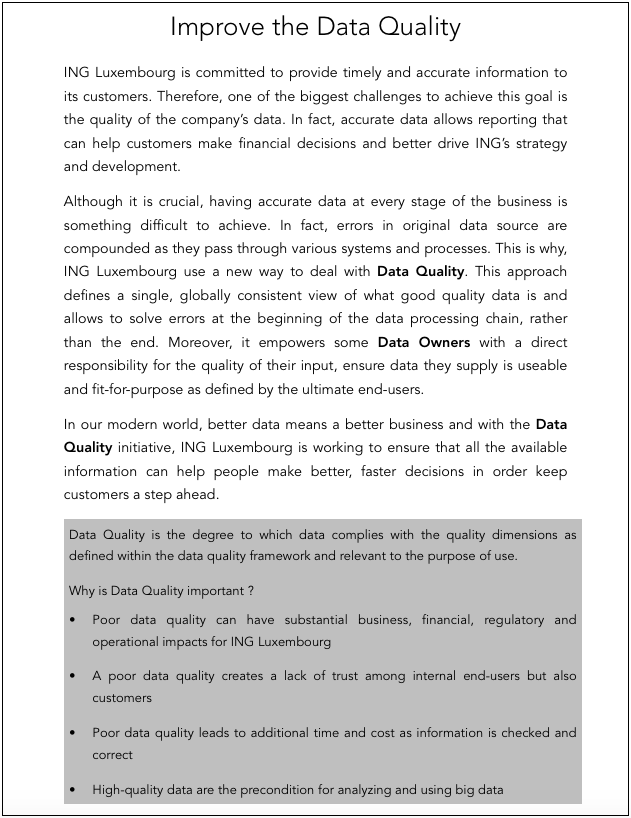
\includegraphics[scale=0.6]{A.png}
\end{center}

\subsection{Liste non-exhaustive des régulations concernant les données dans le secteur financier}

\begin{center}
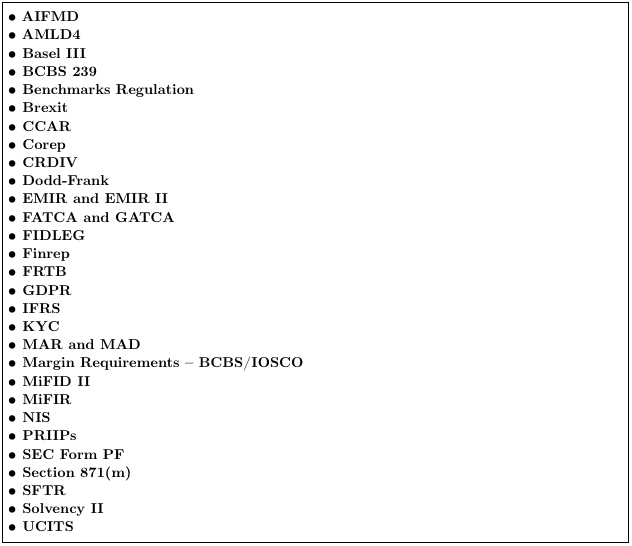
\includegraphics[scale=0.6]{B.png}
\end{center}

\end{document}